
\documentclass{aa}  

\usepackage{graphicx}
%%%%%%%%%%%%%%%%%%%%%%%%%%%%%%%%%%%%%%%%
\usepackage{txfonts}
%%%%%%%%%%%%%%%%%%%%%%%%%%%%%%%%%%%%%%%%
%\usepackage[options]{hyperref}
% To add links in your PDF file, use the package "hyperref"
% with options according to your LaTeX or PDFLaTeX drivers.
%
\begin{document} 


   \title{The data center for X-ray Imaging Spectrometer/Telescope STIX}

   \subtitle{}

   \author{H. Xiao
          \inst{1}
          \and 
          Shane Maloney 
          \inst{2}
          \and 
          Ewan Dickson \inst{1,4}
          \and 
          S\"am Krucker\inst{1}
          \and Andrea Francesco Battaglia\inst{3}
            \and László Etesi \inst{1}
          \and Ryan Daniel \inst{1}
          \and Lastufka Erica \inst{1}
          \and Other STIX team members
         }

   \institute{University of Applied Sciences and Arts Northwestern Switzerland (FHNW), 5200 Windisch, Switzerland \\
              \email{hualin.xiao@fhnw.ch}
         \and
          Astrophysics Research Group, School of Physics, Trinity College Dublin, Dublin 2, Ireland
          \and
             ETH Z\"urich, R\"amistrasse 101, 8092 Z\"urich, Switzerland
         \and University of Graz, Universitätspl. 3, 8010 Graz, Austria
             }

   \date{}

% \abstract{}{}{}{}{} 
% 5 {} token are mandatory
 
  \abstract
  % context heading (optional)
   {} %leave it empty if necessary  
  % {context.}
  % aims heading (mandatory)
   { The Spectrometer/Telescope for Imaging X-rays (STIX) instrument onboard the Solar Orbiter mission launched on February 10, 2020 promises advances in the study of solar flares of various sizes. It is capable of measuring X-ray spectra from 4 to 150 keV with 1 keV resolution binned into 32 energy bins before downlinking. STIX data center is an infrastructure established at FHNW in order to process and archive STIX telemetry data, and to support the operations of the instrument. The automated data processing pipelines turn raw telemetry data into processed information and data products. Processed information and data products are achived at the data center.  STIX data center provides the solar physics community various tools to visualize STIX data products.
   }
  % methods heading (mandatory)
   {Methods}
  % results heading (mandatory)
   {Results.}
  % conclusions heading (optional), leave it empty if necessary 
   {}

   \keywords{Solar flares --Data Center --
                STIX data products --
                Data processing pipeline
               }

   \maketitle
%
%-------------------------------------------------------------------

\section{Introduction}
Solar Orbiter is a Sun-observing mission of the European Space  Agency that 
addresses the interaction between the Sun and the heliosphere.
It was lunched on Feb. 10, 2020 for a nominal mission duration of seven years and a planned 
extension of
three years. It carries ten sets of instruments for comprehensive
remote-sensing and in-situ measurements. 
Solar Orbiter  will perform detailed measurements of the Sun as close as 0.28 AU and for the first time look at its uncharted polar regions (\cite{SolarOrbiter2020}).  
Its goal is to  address the center question of heliophysics  "How does the Sun create and control the heliosphere?".  It is designed to identify the origins and causes of the solar wind, the heliospheric magnetic field, the solar energetic particles, the transient interplanetary disturbances, and the Sun's magnetic field.
This consists of the study of energetic solar phenomena like flares,  solar transients,  the solar wind accelerating mechanisms, and the solar dynamo principle.  


The Spectrometer Telescope for Imaging X-rays (STIX) is one of the ten instruments onboard Solar Orbiter.  It measures X-rays from 4 to 150 keV and takes X-ray images with a few arcsec angular resolution by using an indirect imaging technique, based on the Moiré effect .  It has an angular resolution of 7 arcsec and a spectral resolution of  about 1.0 keV (FWHM) at 30 keV.
STIX instrument consists of 32 collimators with
grids and 32 pixelated Cadmium telluride  detector units called Caliste-SO.
The main science objective of STIX is to study the extremely hot solar plasma and the high-energy electrons accelerated during solar flares. STIX will address the key science goals of the Solar Orbiter mission by providing information on intensity, spectrum, timing, and location of accelerated electrons near the Sun.
For the details of the STIX instrument, we refer to the instrument paper \cite{StixInstrument}.


During nominal science operations, STIX continously acquires data. They are processed and compressed into different types of telemetry packets by
before being tansmitted to the ground.
Being aware of the complexity of the data analysis and of
the need to bring the data to the community, a data center has been
developed at FHNW.
It tasks include receiving, analyzing, archiving and distributing STIX data, and supporting STIX instrument operations.
It turns raw telemetry data into processed information and data products that can be used for scientific analysis.
SDC also provides various data visualization tools to the solar physics comunity.
We will describe here STIX data types,  the flow of data from to the users, the data processing pipelines, the database, the data products and the tools provided for the solar physics comnunity.
%--------------------------------------------------------------------

\section{STIX raw telemetry data}
Data collected from 32 detector units, the aspect system,
housekeeping sensors are processed by the FPGA and the onboard flight software.
They are either processed the onboard FPGA and CPU forming low latency telemetry data or stored in the onboard archive memeory,
which are used to form science data according to requests initiated from the operations team.
STIX sends data to the spacecraft in the form of binary packets.
These data packets are considered as STIX raw telemetry data.
They can be classified into four categories as follows:
\begin{figure}
    \centering
    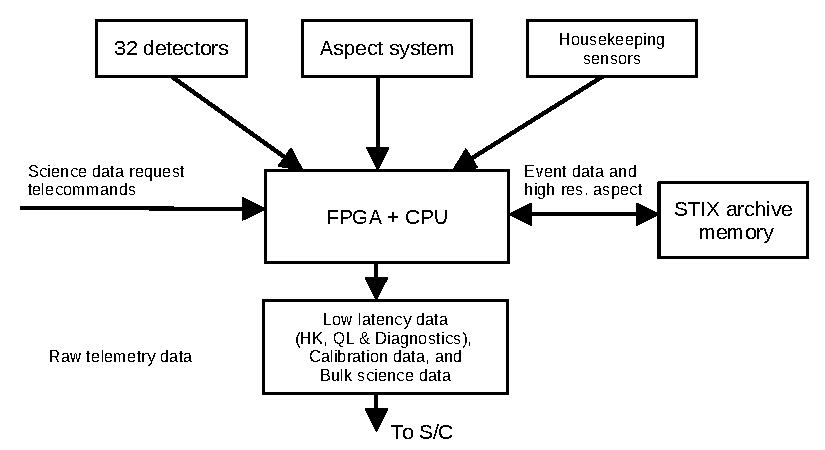
\includegraphics[width=0.8\linewidth]{figures/onboardDataFlow.pdf}
    \caption{STIX onboard data flow and data types.}
    \label{fig:stix_onbard_data_flow}
\end{figure}

\begin{itemize}
 \item  Housekeeping data.
 %STIX generates two different houskeeping data packets.
STIX housekeeping data contain engineering  data that measure temperatures, voltages, currents, status of switches,
averaged signal readouts from the four aspect photodiodes, detector trigger counts and  flags indicating
status of the onboard software.
They are generated as long as STIX is powered on.
The housekeeping packet generation candence is adjustable by telecommands.
During nominal operations, the HK generate candence is configured to 64 sec / packet and
the HK data rate is 143 kiB / day.
HK data arrive at STIX data center with latencies ranging from a few minutes to days, depending on whether
it is in a data-link pass.

\item Quick-look (QL) data.
STIX generates four different types of quick-look data in NOMINAL mode: light curves, background light curves, energy spectra and variance.
Quick-look light curves are  time series of counts
of all pixels in 30 detectors (excluding background detector and the coarse flare locator)
accumulated every a few seconds (4 sec nominal) in five different energy ranges.
Background light curves are similar to the Quick-look light curves but only
counts recorded by the background detector are included.
Variance data are
the detector-summed variance of count rates
based on 0.1s integration.
Quick-look spectra are snapshots of energy spectra for for each of the 32 detectors.
Nominally, STIX acquires an energy spectrum (32 seconds integration time) for each channel every 17 minutes.

\item
Calibration data. When STIX is NOMINAL mode, high-resolution calibration spectra  are accumulated for events from the weak onboard $^{133}$Ba
radioactive sources during solar quiet  (non-flaring)  times. The relevant portions of these
spectra are routinely included in the quick-look low-latency data.
The nominal accumulation time is 24 hours.

\item
Science data.  The science data are different combination of summing and compression of the basic pixel data stored in the archive memoery.
Each science request can selects subsets of of energies, pixels and detectors.
They are generated when  STIX executes
science data request commands which are initiated from the STIX operations team. Science data have six different types : 1)
Level-0 X-ray data is the least processed data and contains uncompressed counts for the selected energies, pixels and detectors.
2) Level-1 is essentially the same as Level-0 but the counts are compressed on-board before being sent to ground.
3) For Level-2 data,  counts from the 12 pixel are summed down to 4 before compression.
4) Level-3 are visibilities, which further reduces the data by combine the the 4 summed pixel counts into a complex visibility which is also compressed.
5) Level-3 are spectrograms, which combines spectra of all selected pixels.
6) High time resolution aspect data.
\end{itemize}

The first three categories are  transferred to the
common low latency data store in SSMM.

Table \ref{tb:raw_types} shows a summary of telemetry packets.

\begin{table}[h]
\caption{STIX raw telemetry packet types.}
\begin{tabular}{lllll}
\hline
Category & Type & & & \\ \hline
Quicklook    & light curves           &  &  &  \\ \hline
Science      & L1, L2, L3, L4, aspect &  &  &  \\ \hline
Housekeeping & Housekeeping           &  &  &  \\ \hline
Calibration  & calibration            &  &  &  \\ \hline
\end{tabular}
\label{raw_types}
\end{table}

The latency of
During the nomal operation, STIX continously collects data from the 32 x-ray detector units, the aspect system and
housekeeping sensors. The collected data are processed by a FPGA and flight software running on a soft CPU core.
The processed data are directed to the low latency data store in SSMM or stored in STIX
onboard archive memory.  The data stored in the onboard archive memeory can
be processed and form science data on requests from the ground.

 HK and QL will be
directed to the Low Latency data store in SSMM.



\section{Data link and data reception}
For the most part, STIX data are organized by data content, with each major data content
type (e.g. x-ray imaging data, spatially-averaged x-ray data, HK data, etc.) associated with
its own packet types. While the format of each packet type is fixed, the relative frequency of
each packet type is dependent on solar activity and/or instrument mode. Although the mix
of packet types will vary, the 1-day average of HK and QL will respect the allocated rate of
4.3 Mbits/day (50 bps) each. The sum of all data types will respect the orbital average of 1.8
Gbits/orbit (700 bits/second for 30 days). STIX can make use of an on-board memory to
load the SSMM at a rate compatible with spacecraft requirements.

During nominal science operations, science data are downlinked for eight hours during each
communication period with the ground stations. Additional eight-hour downlink passes are
scheduled as needed to reach the required total science data return of the mission.
The Solar Orbiter ground segment makes maximum reuse of ESA's infrastructure for Deep Space missions:

The ground stations, which belong to ESA's space tracking station network (ESTRACK)
The Mission Operations Centre (MOC), located at ESOC, Darmstadt, Germany
The Science Operations Centre (SOC), located at ESAC, Villanueva de la Cañada, Spain
The communications network, linking the various remotely located centres and stations to support the operational data traffic
The Science Operations Centre was responsible for mission planning and the generation of payload operations requests to the MOC, as well as science data archiving. The SOC has been operational for the active science phase of the mission, i.e. from the beginning of the Cruise Phase onwards. The handover of payload operations from the MOC to the SOC is performed at the end of the Near-Earth Commissioning Phase (NECP). ESA's Malargüe Station in Argentina will be used for all operations throughout the mission, with the ground stations of New Norcia Station, Australia, and Cebreros Station, Spain, acting as backup when necessary.[12] wikipedia

STIX telemetry data are firstly stored in the spacecraft solid state disk (SSMM).
Low latency telemetry data are downlinked  with the ground stations during each communication period with the ground stations.
Science data are downloaded  as needed to reach the required total science data return of the mission.

They are transmitted to ground stations during antenna passes.
Telemetry data recieved by ground stations are processed at the mission control center of ESA and
stored in .
ESA provides a web interface.
The typical latency of the low latency data before they arrive at STIX data center is about x day when there is a pass a.
Raw data received at STIX data center has the same structure.

The payload data must be created through the EEDS web page to create a data download request.
After receiving the user's data request, EDDS displays the original payload data in the form of hex code and sends it to the stix data center server through the RSYNC protocol. Users can define the time interval of data request. Generally speaking, STIX server requests data from EDDS once a day. The data STIX obtains from EDDS is a HEX code with a time stamp, which is the same as the data sent by STIX to the spacecraft platform after being converted into binary data.
In addition to telemetry data, STIX data center also receive spacecraft ancillary data from
the mission operation center, which contains
information of spacecraft ephemris and factors for time conversion.


\section{Data processing pipelines at STIX data center}


\section{Filename naming conventions}

\subsection{STIX raw data processing pipeline}
\subsubsection{Raw data parsing}

include a decompression error map here

\subsection{metadata and sysposis data creation}

\subsubsection{FITS file creation}



\subsubsection{Background data processing pipeline}
Light curves measured during quiet periods of the sun are used for background estimation. Median values and of counts are computed and considered as the background in the selected time frame. They are stored in a database and used for flare identifications. 

\subsection{Calibration data processing pipeline}
The calibration data processing pipeline is started automatically after the calibration data raw packets
are being parsed and written to the NoSQL database.


As described in Ref. \cite{StixInstrument},  Ba134 radioactive sources with a total activity of about 4000 Bq are placed at the front of each detector. The total activity of the radioactive source is approximately 4000 Ba.
When the radioactive source decays, gamma rays are generated. These gamma rays can form peaks in the energy spectrum of the detector.
As the energies of the peaks are known, and the corresponding relationship between ADC and real energy can be calibrated through the position of the peak in the energy spectrum, that is, the calibration coefficient. The figure below is a typical Ba133 gamma-ray energy spectrum measured by STIX CdTe detector. There are three obvious peaks in the energy spectrum, and they correspond to three energies of 30 keV, 35 keV and 81 keV. There are many ways to determine the position of each peak, you can use the ECC method, or use the Gaussian function to fit the left part of the peak.


ELUT and calibratino factors can be downloaded from STIX data center by using web GUIs or python APIs.
\subsubsection{calibration analysis production, ELUT}

\section{Data request procedure}

For detected flares,  a script is used to create data requests.
If the background subtracted peak count rate of a flare is greater 150,
both L1 and spectrogram rquests are created;  For microflares, as only
spectrograms are request normally as the statistics is too
low to recontruct flare images.  Aspect data requests
and some extra data requests are created for events of interest by the
STIX operations team.
For external users, data request forms can be also submitted using a web tool
at the data center.

An unique ID is assigned to each data request automatically.
The ID naming convention is yyddmmxxxx, in which yyddmm indicate the observation year (without century), month, date,
and the last four digits indicates the serial number of the data request in the day.
IDs are used to track the status of data requests, and reterieve data products from the
STIX data center.
The information of created data requests are stored in the NoSQL database on the same server.
They are converted to instrument operation requests (IORs) after a series of checks.
Requested data will arrive at STIX data center within a time frame of two weeks to three months, depending on
telemetry allocations.


\section{Flare processing pipeline}

\subsubsection{Flare identification}
Quick-look light curves in the energy range 4 to 10 keV are used for solar flare identification.  The flare identification procedure consists of  two steps:
\begin{itemize}
\item Light curve smoothing. In order to filter spikes from electronics and to reduce the amount of variation due to statistics and the onboard integer compression, light curves are smoothed by using the average filtering. The
\item Flare identification. Local maximums are selected from smoothed light curves.  A local maximum is considered as a flare peak if the counts are exceeds 2 standard deviations above the background and the duration above the background is longer than 1 minute.
\end{itemize}

For each of identified solar flares,   the  information such as start time, end time, counts, background subtracted counts is stored in the STIX flare database.   It is used for automatic creation of data requests for on-board archived data.

How to define a flux.


\subsubsection{flare ID naming convention}
\subsubsection{Flare locations}

\subsection{Solar flare list}
\subsection{Flare location database}


A list of products from the flare processing pipeline

* Flare list
* Flare location
*

\subsubsection{Flare location using coarse flare data}
\subsubsection{Flare classification using GOES x-ray flux}

\section{STIX data products}

\subsection{L1 data products}
\begin{itemize}
    \item Raw data.
    \item L1 data.
    \item L2 data
    
\end{itemize}

The latest level 1 FITS IO from Shane has been integrated into the data processing pipeline on pub023 server.

I have recreated fits products for all old telemetry data with the upgraded SW.

The L1 fits files  created by this pipeline have a different data level:  L1A ('A' here means  prerelease/alpha version).

The idea behind L1A data sets is to allow for quicker access to STIX data in the fits format instead of grabbing  data from plots or using JSON requests,

for operations,  debugging  etc.

The L1A data sets can be generated within a few minutes after the arrival of a new raw telemetry file.

The differences between L1A and L1 available in Shane's ftp include:

1.  Two different L1A data files may have duplicated data

2.  L1A data sets are still created for incomplete packets  (L1 checks for data completeness)

3.  SPICE kernel data for telemetry files always arrives  after one or two days later.
    So  there may be a sub-second difference between the UTC time in fits files (same to times on web pages)

   and the real time.

    Shane's formal L1 release can avoid this issue if they are produced on a later date.

4. L1A contains housekeeping data

The different data-processing levels for HMI are summarized as follows, with more details available from this source:
• Data at Level 0 are images that have been constructed from the raw telemetry stream.
• Data at Level 1.0 are images that have been converted from Level 0, with processing including bad-pixel removal, flat-fielding,
and quality assessment checks, but otherwise not having undergone any irreversible data alterations.
• Data at Level 1.5 are images of the physical observables (Dopplergrams, magnetograms, and continuum images), which were
constructed from the individual Level 1.0 filtergrams.
• Data at Level 2 have been irrevocably filtered, time-sequence-merged, Fourier-transformed or otherwise changed from Level 1.5
data in a way that is irreversible. Level 2 products include intermediate products for later production of mission science data
products, such as helioseismic inferences of solar subsurface flows


The Level0 archive contains TM which has been parsed or decommuated into readable structures but no additional external information is include:

times are not converted to UTC
no calibration or conversions applied
for STIX we need to decide if we decompress / combine X-ray L0 the count/trigger data at this stage or in the next level L1

copy manual,
tree like, 
json formats
name, raw value, eng value, children
look-up table, to know description

estimate mongodb benchmark
Mongodb benchmark,
key value, index, performance


\subsection{Auxilary data}



\begin{table}
\centering
\caption{Level 1 data products}
\begin{tabular}{llll}
Category & Type   &  Naming convention  & Remarks   \\ \hline
 Housekeeping & hk\_mini  &  & Houskeeping in BOOT mode   \\
 & hk\_maxi  &  & houskeeping data in NOMINAL   \\
 Quick-look &  light curves &  & Quicklook lightcurves \\
  &  variance &  & variance \\
  &  spectra &  &  \\
  &  background monitor &  &  \\
    &  flare location &  &  \\
 Calibration data &   &  &  \\
\end{tabular}
\end{table}


\section{Database}
\subsection{Raw data packet database } 
\subsection{Configuration database}

\section{Online data visualization tools}
\subsection{Quick-look light curve}
\subsection{Science data quick analysis}
\subsubsection{Calibration data}
\begin{figure}
    \centering
    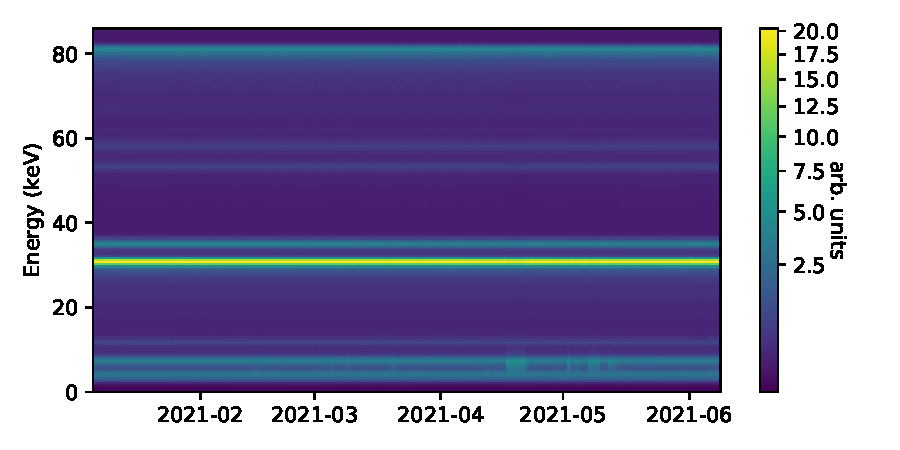
\includegraphics[width=0.8\linewidth]{figures/calibrationSpectrogram.pdf}
    \caption{Caption}
    \label{fig:calibrationSpectrum}
\end{figure}
\begin{figure}
    \centering
    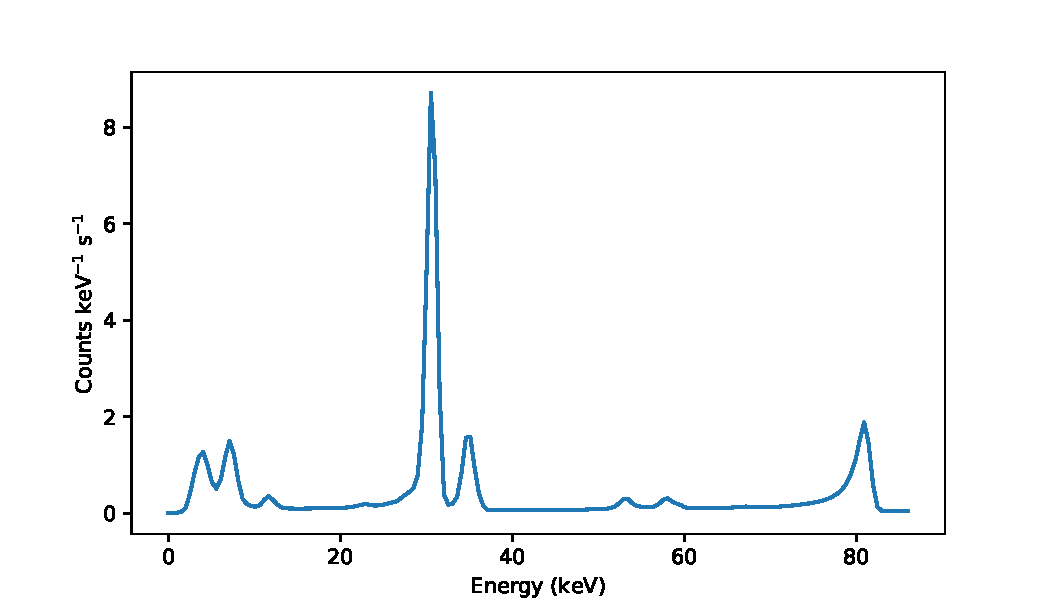
\includegraphics[width=0.8\linewidth]{figures/calibrationSpectrum.pdf}
    \caption{Spectrogram of STIX calibration spectra}
    \label{fig:calibrationSpectrogram}
\end{figure}

calibration data products
https://fermi.gsfc.nasa.gov/ssc/data/access/gbm/
\subsubsection{Solar Orbiter orbit viewer}


When a new data file from the platform is received at the PPDC,
it triggers an autonomous start of the dedicated program that decodes and
interprets its contents. The binary data contain the spacecraft location, attitude, speed, and GPS timestamps with increments every half second. The GPS timestamps are converted into Unix-timestamps, where the leap seconds are also considered. After processing, the platform data are written to the ROOT format files. The data start and stop time, data processing time, input filename and ID of the output file of each processing are recorded in a dedicated database table.
SPICE kernel

Updated once per day.

At the center of the Sun.
It is worth mentioning that has to corrected for.
This can be done by using the web tool provided at the auxiliary data center at

\subsection{Automated data request scheme}
scheme


\section{Data access and APIs}
\section{Future work}
\section{Conclusions}



% WARNING
%-------------------------------------------------------------------
% Please note that we have included the references to the file aa.dem in
% order to compile it, but we ask you to:
%
% - use BibTeX with the regular commands:
%   \bibliographystyle{aa} % style aa.bst
%   \bibliography{Yourfile} % your references Yourfile.bib
%
% - join the .bib files when you upload your source files
%-------------------------------------------------------------------

\bibliographystyle{aa}
\bibliography{citations}

\end{document}
